\documentclass{exam}

\usepackage{units} 
\usepackage{graphicx}
\usepackage[fleqn]{amsmath}
\usepackage{cancel}
\usepackage{float}
\usepackage{mdwlist}
\usepackage{booktabs}
\usepackage{cancel}
\usepackage{polynom}
\usepackage{caption}
\usepackage{fullpage}
\usepackage{xfrac}
\usepackage{enumerate}

\newcommand{\degree}{\ensuremath{^\circ}} 
\everymath{\displaystyle}

\printanswers

% \begin{figure}[H]
%   \centering
%   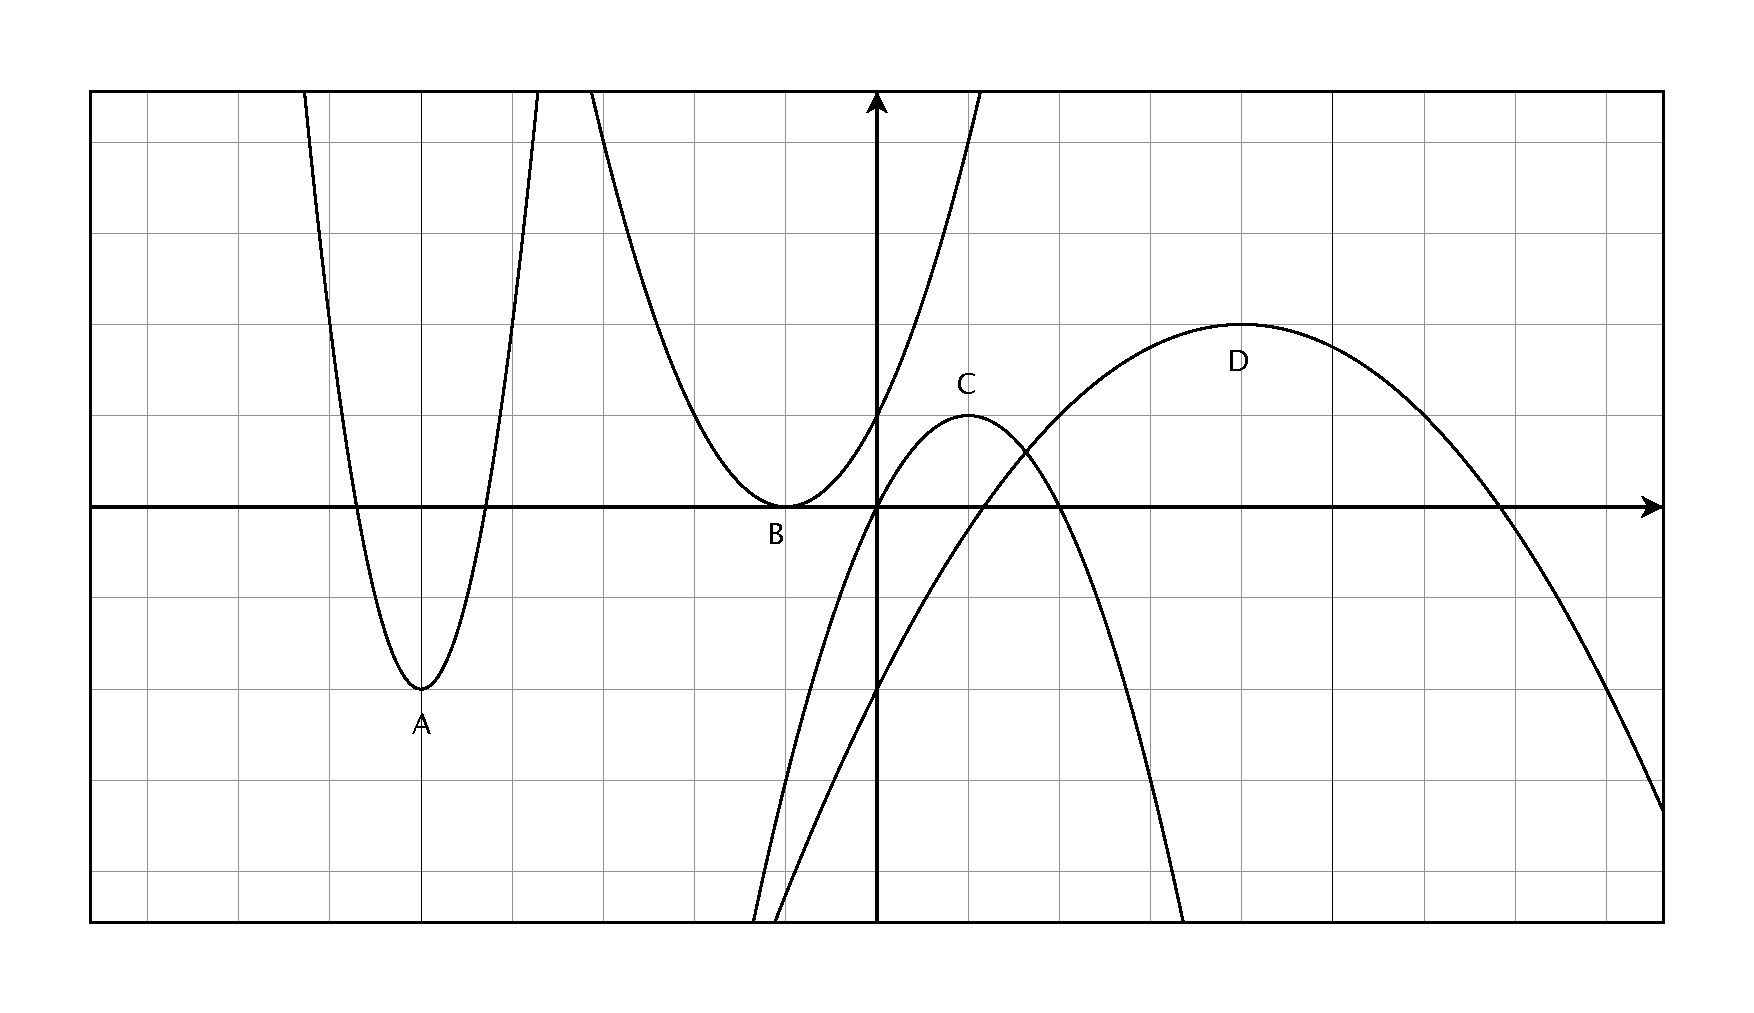
\includegraphics[scale=.3]{problem_7.eps}
%   \caption*{Problem 7}
% \end{figure}

% \begin{tabular}{cc}
% \toprule
% period & amplitude \\
% \midrule
%   $\pi$ & $2$ \\
% \bottomrule
% \end{tabular}

\title{Math 141 Notes \\ Section 4.3}

\date{June 19, 2013}

\begin{document}

  \maketitle
  \tableofcontents

  \section{Rules of Exponents}

  \begin{align*}
    x^a \cdot x^b        &= x^{a + b} \\
    \frac{x^a}{x^b}      &= x^{a - b} \\
    \left( x^a \right)^b &= x^{ab} \\
  \end{align*}

  \section{Rules of Logarithms}

  \begin{align*}
    m &= b^x \\
    x &= \log_b m \\
    \\
    n &= b^y \\
    y &= \log_b n \\
  \end{align*}

  multiplying
  \begin{align*}
    \log_b \left( mn \right) &= \log_b \left( b^x \cdot b^y \right)
                             &= \log_b b^{x + y} \\
                             &= x + y \\
                             &= \log_b m + \log_b n \\
  \end{align*}

  dividing
  \begin{align*}
    \log_b \left( \frac{m}{n} \right) &= \log_b \left( \frac{b^x}{b^y} \right)
                             &= \log_b b^{x - y} \\
                             &= x i y \\
                             &= \log_b m - \log_b n \\
  \end{align*}

\end{document}
